\documentclass[a4paper,12pt]{article}
\usepackage{HomeWorkTemplate}

\usepackage[utf8]{inputenc}
\usepackage[]{babel}

\setlength{\parindent}{4em}
\setlength{\parskip}{0.5em}

\renewcommand{\baselinestretch}{1.5}

\usepackage{caption}
\usepackage{subcaption}
\usepackage{float}
\usepackage{amsmath}
\usepackage[utf8]{inputenc}
\usepackage{lmodern, textcomp}
\usepackage{circuitikz}
\usepackage[shortlabels]{enumitem}
\usepackage{hyperref}
\usepackage{tikz}
\usepackage{amsmath}
\usepackage{amssymb}
\usepackage{tcolorbox}
\usepackage{graphicx}
\usepackage{xepersian}
\settextfont{XB Niloofar}
\usetikzlibrary{arrows,automata}
\usetikzlibrary{circuits.logic.US}
\usepackage{changepage}
\newcounter{problemcounter}
\newcounter{subproblemcounter}
\setcounter{problemcounter}{1}
\setcounter{subproblemcounter}{1}
\newcommand{\problem}[1]
{
	\subsection*{
		پرسش
		\arabic{problemcounter} 
		\stepcounter{problemcounter}
		\setcounter{subproblemcounter}{1}
		#1
	}
}
\newcommand{\subproblem}{
	\textbf{\harfi{subproblemcounter})}\stepcounter{subproblemcounter}
}


\begin{document}
\handout
{اصول پردازش تصویر}
{دکتر مصطفی کمالی تبریزی}
{نیم‌سال اول 1399\lr{-}1400}
{اطلاعیه}
{سیدعلیرضا خادم}
{97100398}
{تمرین سری سوم - سوال سوم}
زمان حدودی اجرا برای 2048 سگمنت و تصویر با سایز اصلی : 15 ثانیه
\section*{موارد لازم.}
برای اجرا لازم است تا تصویر
 \lr{slic.jpg}
در مسیر
\lr{EX3\_Q2/images/}
قرار داشته باشد. همچنین در پیاده‌سازی این سوال از کتابخانه‌های 
\lr{numpy}
،
\lr{skimage}
و
\lr{cv2}
استفاده شده است که قبل از اجرا بایستی این کتابخانه‌ها روی سیستم شما نصب باشد.
\section*{روند کلی حل.}
ایده کلی الگوریتم 
\lr{slic}
بسیار مشابه الگوریتم 
\lr{Turbo pixel}
است و به این صورت است که در ابتدا تعداد کلاسترهایی که میخواهیم در نهایت داشته باشیم را در نظر می‌گیریم و مرکز این کلاسترها را به صورت یونیفرم در تصویر پخش می‌کنیم. قبل از هر کاری در ابتدا هر یک از این 
\lr{cluster center}
ها در یک پنجره‌ای به ابعاد 11 در 11 به مرکزیت خودشان جابه‌جا می‌شوند تا در مکانی از این پنجره که کمترین گرادیان را دارد قرار بگیرند. بعد پیکسل‌های اطراف هر کدام از این کلاستر سنترها بر اساس معیار‌هایی که در روابط زیر مشاهده می‌کنید به کلاستر سنترها اختصاص می‌دهیم.
\begin{figure}[H]
	\centering
	\begin{subfigure}{0.6\textwidth}
		\centering
		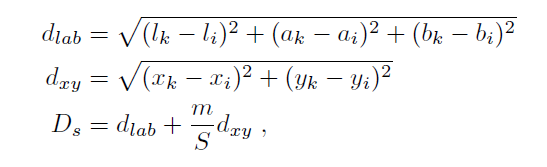
\includegraphics[width=\textwidth]{1.png}
	\end{subfigure}
\end{figure}
در رابطه بالا 
\lr{S}
فاصله دو کلاستر سنتر بعد از توزیع یکنواخت آنها روی تصویر است و ما در این سوال 
\lr{m}
را مساوی 22 در نظر گرفته‌ایم.\\\\
پیاده‌سازی‌ای که در این کد صورت گرفته است تا حدی زیادی مشابه توضیحاتی است که در صورت سوال آمده است اما تفاوت‌هایی هم با آن دارد که این تفاوت‌ها عبارت اند از :	 در روشی که در صورت سوال آمده است یک آستانه برای اختصاص دادنِ یک پیکسل به یک کلاستر در نظر گرفته شده است به طوری که اگر 
$ D_s = d_{lab} + \dfrac{22}{S}d_{xy} $
از آن آستانه کمتر باشد به آن کلاستر سنتر اختصاص داده می‌شود. در این روش امکان این که تعدادی پیکسل در نتیجه نهایی به هیچ کلاستری اختصاص داده نشوند یا به چند کلاستر اختصاص داده شوند وجود دارد، اما پیاده سازی‌ای که در این کد انجام شده است به این صورت است که کلاستر سنترها را از گوشه چپ بالا پیمایش میکنم و در هر گام پیمایش پنجره‌ای به ابعاد $ 2S *‌2S $ پیرامون کلاستر سنتر در نظر می‌گیریم و مقدار $ D_s $ را برای هر پیکسل در این پنجره و کلاستر سنتری که در حال حاضر روی آن قرار داریم محاسبه میکنیم. آرایه‌
\lr{data}
 را به ابعاد 
$ image\_height *‌ image\_width *‌ 2 $
در نظر می‌گیریم به گونه‌ای که $ data[x,y,0] $ نشان‌ میدهد که پیکسل $ x,y $ آخرین بار به کدام کلاستر اختصاص داده شده است و $ data[x,y,1] $ نشان می‌دهد $ D_s $ دراختصاص این پیکسل به 
$ data[x,y,0]$
چقدر بوده است. در ابتدا همه داریه‌های $ data $ را با مقدار $ np.inf $ مقداردهی می‌کنیم. در  هر گام از پیمایش کلاسترها اگر پیکسل $ ِD_s $ ای که دارد از $ data[x,y,1] $ 
کمتر باشد به این معنی است که این پیکسل بیشتر به این کلاستر نزدیک است تا $ data[x,y,0] $ ؛ در نتیجه مقادیر 
$ data[x,y,0] $
و
$ data[x,y,1] $
را آپدیت می‌کنیم. هر بار که یک پیکسل به یک کلاستر اختصاص داده می‌شود، مقدار کلاستر سنتر متناظر را آپدیت ‌می‌کنیم.



\section*{توضیح کد.}
برنامه در مجموع حاوی 2 فایل با فرمت
\lr{.py}
می‌باشد که توضیحات هر فایل در پایین آمده است.
\subsection*{$\circ$ utilities.py}
\subsubsection*{\lr{resize\_image(src\_image, scale)}}
این  تابع یک تصویر یک عدد (‌برحسب درصد) به بعوان ورودی می‌گیرد و طول و عرض تصویر را با نسبت داده شده تغییر می‌دهد و عکس تغییرسایز داده‌شده را به عنوان خروجی بر‌می‌گرداند.
\subsubsection*{\lr{apply\_sobel\_filter\_x(gray\_image)}}
این تابع یک تصویر سیاه سفید را به عنوان ورودی می‌گیرد و فیلتر sobel\_x را برای پیدا کردن مرزهای عمودی روی تصویر اعمال می‌کند و نتیجه را به عنوان خروجی بر‌می‌گرداند.
\subsubsection*{\lr{apply\_sobel\_filter\_y(gray\_image)}}
این تابع یک تصویر سیاه سفید را به عنوان ورودی می‌گیرد و فیلتر sobel\_y را برای پیدا کردن مرزهای افقی روی تصویر اعمال می‌کند و نتیجه را به عنوان خروجی بر‌می‌گرداند.
\subsubsection*{\lr{get\_edges(src\_image)}}
این تابع یک تصویر را به عنوان ورودی می‌گیرد و بعد از آنکه آن را به تصویر سیاه‌سفید تبدیل با استفاده از توابع \\
\lr{apply\_sobel\_filter\_x(gray\_image)} و \lr{apply\_sobel\_filter\_y(gray\_image)}
مرزهای تصویر سیاه‌سفید شده را به دست می‌آورد و به عنوان خروجی بر‌می‌گرداند.
\subsubsection*{\lr{initialize\_cluster\_centers(...)}}
این تابع با استفاده از ورودی‌هایی که می‌گیرد مختصات کلاستر سنترها را محاسبه می‌کند، به گونه‌ای که توزیع کلاستر سنترها یونیفرم باشد و فاصله هر کلاستر سنتر با کلاستر سنتر مجاور آن S باشد.
\subsubsection*{\lr{perturb\_cluster\_centers(cluster\_centers, src\_image\_edges, indexes)}}
این تابع کلاستر سنترها ، تصویر مرزها و ماتریس 
\lr{indexes}
را به عنوان ورودی می‌گیرد سپس در پنجره‌ای با ابعاد 
\lr{indexes}
(11 * 11)
هر یک از کلاستر سنترها را به گونه‌ای جابه‌جا میکند تا در مختصاتی با کمترین گرایان در این پنجره قرار بگیرند.
\subsubsection*{\lr{cal\_dist(cluster\_center, pixel\_x, pixel\_y, scaled\_image, S)}}
این تابع یک کلاستر سنتر ، مختصات یک پیکسل و S را به عنوان ورودی می‌گیرد و با توجه به روابط زیر معیاری از میزان فاصله‌ی این پیکسل از آن کلاستر سنتر را در فضای 
$ [x, y, l, a, b] $
محاسبه می‌کند و به عنوان خروجی برمی‌گرداند.
\begin{figure}[H]
	\centering
	\begin{subfigure}{0.5\textwidth}
		\centering
		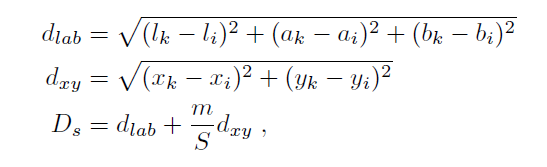
\includegraphics[width=\textwidth]{1.png}
	\end{subfigure}
\end{figure}
\subsubsection*{\lr{slic(cluster\_centers, scaled\_image, S, f, data, segments=None)}}
این تابع تمامی موارد در قسمت 
\textbf{روند کلی حل.}
شده است را پیاده سازی می‌کند. در ابتدا محاسبات به صورت پیمایش روی پیکسل‌های پنجره $ 2S * 2S $ با فور انجام می‌شد که بسیار از نظر زمانی کند بود. در راستای بهبود سرعت این تابع محسابات به صورت ماتریسی انجام شد که سرعت اجرای کد را حدود 60 برابر بهتر کرد.
\subsubsection*{\lr{draw\_boundaries(segments, scaled\_image)}}
این تابع سگمنت‌ها و تصویرِ تغییرسایز داده شده را به عنوان ورودی می‌گیرد و با استفاده از تابع 
\lr{find\_boundaries}
از کتابخانه 
\lr{skimage}
مرزهای سگمنت‌ها را به دست می‌آورد و مقدار 
\lr{intensity}
پیکسل‌های مرزها 255 قرار می‌دهد تا مرز سگمنت‌ها در تصویر مشخص شود.
\subsubsection*{$\circ$ q3.py}
در این فایل ابتدا تعداد کلاسترها و $ scale $ تغییر سایز تصویر با استفاده از تابع 
\lr{get\_input}
از ورودی گرفته می‌شود و به ترتیب در متغیرهای 
\lr{num\_of\_clusters}
و
\lr{scale}
ذخیره ‌می‌کنیم.در ادامه تصویر 
\lr{slic.jpg}
را از مسیر 
\lr{EX3\_Q3/images/}
لود میکنم و فضای رنگی آن را به 
$ LAB$
تبدیل کرده و در متغیر
\lr{lab\_image}
ذخیره می‌کنیم(البته قبل از تبدیل کردن فضای رنگی، فیلتر 
\lr{bilateral}
روی تصور اعمال می‌کنیم تا نویز‌ در تصویر نهایی کمتر باشد.) تصویر را در ادامه با 
\lr{scale}‌ای 
که به عنوان ورودی از کاربرگرفته شده است ریسایز می‌کنیم، کلاستر سنتر‌ها را 
\lr{initialize}
می‌کنیم تا به صورت یونیفرم در تصویر پخش شوند، ماتریس f را به گونه‌ای میسازیم که درایه‌ی $ i, j $ آن
$ i-S, j-S $
باشد (از این ماتریس در تابع 
\lr{slic}
استفاده میکنیم تا بدون فور بتوانیم پنجره $ 2S * 2S $ را محاسبه کنیم
)
در نهایت هم با استفاده از تابع slic که در فایل utilities.py پیاده‌سازی شده سگمنت‌ها را به دست می‌آوریم و با تابع draw\_boundaries مرز سگمنت‌ها را رسم می‌کنیم و نتیجه را با نام test.jpg در مسیر 
\lr{EX3\_Q3/results/}
ذخیره می‌کنیم.


\end{document}
